    \section{Introduction}\label{sec:intro}
% Introduce the topic
Image captioning models take advantage of correlations between co-occurring captions and images in the training data. Therefore, the presence of societal biases in the large-scale datasets on which these models are trained can cause these models to not only reproduce the inequalities in the datasets but also amplify them \cite{zhao}. %\\

% Introduce the paper + our work
\citeauthor{hirota} investigate this problem in the paper \citetitle{hirota}.
%In their paper \textit{Quantifying Societal Bias Amplification in Image Captioning} \cite{hirota}, Hirota et al. investigate this problem. 
They argue that existing bias amplification metrics, including Bias Amplification (BA) \cite{zhao} and Leakage \cite{leakage}, are insufficient when applied to image captioning. Therefore, they propose a new metric to specifically study bias amplification in image captioning, called Leakage for Image Captioning (LIC).  It is built on top of the idea that a model amplifies societal bias if a classifier can predict the protected attributes\footnote{\textit{Protected attribute} refers to a demographic variable like age, gender or race that a model should not use to produce an output.} values (e.g.\ female, male) more accurately from the generated captions than from human captions. 

The authors use this metric to conduct extensive evaluation on both traditional and state-of-the-art image captioning models. In this work, we aim to verify their main claims by reproducing their main findings. Furthermore, we extend upon their work by evaluating LIC for age as a protected attribute. This subsequent experiment allows us to assess the generalizability of LIC for other protected attributes, as well as its overall robustness.
 % \\

% Describe the structure of our paper
The remainder of this work will be structured as follows: first, we identify the main claims from the original paper in Section \ref{sec:scope}. Section \ref{sec:methods} outlines our approach towards verifying these claims and extending upon the original work through reproduction and additional experimentation respectively. We give an overview of our experimental results in Section \ref{sec:results}. Finally, we discuss these results and our experience with reproducing and extending the paper in Section \ref{sec:discussion}.

\section{Scope of reproducibility}
\label{sec:scope}
\citeauthor{hirota} study bias amplification on captions generated by various image captioning models. %such as but not limited to NIC \cite{nic} and Att2in \cite{fc_att2in}.
%, include NIC+ and NIC+Equalizer \cite{nic_plus} among others, the latter of which uses a gender equalizer designed to reduce gender bias.
The LIC score for these models is evaluated on a captions dataset with binary gender and race annotations \cite{annotations}. Furthermore, three language encoders \cite{bert, lstm} 
are used for encoding captions in order to evaluate LIC's robustness against changes in sentence representation. The reader is invited to study Section \ref{sec:methods} for implementation-specific details. We use the provided methodology and source code in order to verify the authors' main claims:

\begin{itemize}
    \item \textit{Claim 1}: All the models amplify gender bias.
    \item \textit{Claim 2}: All the models amplify racial bias.
    \item \textit{Claim 3}: LIC is robust against encoders.
    \item \textit{Claim 4}: NIC+Equalizer increases gender bias with respect to the baseline NIC+.
\end{itemize}

Upon verifying these claims, 
we take a step further and evaluate the LIC metric in the context of another type of bias, namely age bias. We specifically use age as additional protected attribute because mentions of age are likely to appear in the available captions dataset. This opens up a new possibility to assess the LIC metric. 

\section{Methodology}
\label{sec:methods}
%Explain your approach - did you use the author's code, or did you aim to re-implement the approach from the description in the paper? Summarize the resources (code, documentation, GPUs) that you used.

\subsection{Calculating the LIC score}

Hirota et al.\ \cite{hirota} use Leakage for Image Captioning (LIC) as a metric to measure bias amplification in image captioning models. 
In order to evaluate the LIC score for a model $M$, one needs to have access to a training set $D$ and test set $D'$ with samples ($I$, $y$, $\hat{y}$, $a$), where $I$ is an image, $y$ is a human caption, $\hat{y} = M(I)$ is a generated caption and $a$ is the protected attributes value. Then the LIC score is calculated as follows. %\\

First, all captions are preprocessed by masking words related to the protected attribute. Details about the preprocessing are found in Section \ref{ssec:datasets}.

Second, two classifiers are trained to predict the protected attribute from a masked caption. The first classifier $f$ is trained on the human captions in the train set $D$, while the second classifier $\hat{f}$ is trained on the generated captions. Both classifiers rely on a natural language encoder, which also needs to be learned on the training data. Let us denote the confidence score of the first classifier as $s_a$. Then this classifier predicts the protected attribute $a$ from a caption $y$ as 

\begin{equation}
    \hat{a} = f(y) = \arg\max_a s_a (E(y))
\end{equation}

where $E$ is the natural language encoder. The same applies for $\hat{f}$, $\hat{E}$, $\hat{s}_a$ and $\hat{y}$ in case of the second classifier. %\\

After the classifiers are trained, they are evaluated on the corresponding test sets of human and generated captions. LIC is built on top of the hypothesis that in an unbiased set of captions, there should not exist differences between how demographic groups are represented. Thus, if a classifier was trained on an unbiased dataset, it could not have learnt how to correctly predict the protected attribute of a masked caption. The higher the accuracy and confidence scores of the predictions, the more biased the captions are. From the evaluation of the first classifier on the test set, the bias in the human captions can then be quantified as

\begin{equation}
    LIC_D = \frac{1}{|\mathcal{D'}|} \sum_{(y,a) \in \mathcal{D'}} s_a (y) \mathbb{1}[f(y) = a]
\end{equation}

where $\mathbb{1}[\cdot]$ is the indicator function. Similarly, from the evaluation of the second classifier on the test set, the bias in the generated captions can be quantified as 

\begin{equation}
    LIC_M = \frac{1}{|\mathcal{D'}|} \sum_{(\hat{y},a) \in \mathcal{D'}} \hat{s}_a (\hat{y}) \mathbb{1}[\hat{f}(\hat{y}) = a].
\end{equation}

Finally, the LIC score is calculated as the amount of bias introduced by the model with respect to the human captions:

\begin{equation}
    LIC = LIC_M - LIC_D.
\end{equation}

A model amplifies bias if LIC > 0 and mitigates it otherwise.

\subsection{Model descriptions}
% describe classifiers used (highlight diff between nic+ and equalizer)
% Three types of models are used to reproduce the experiments: captioning models, sentence classifiers, and language encoders. The relevance of these models is described in the following section.
We describe the model types (captioning models, sentence classifiers, and language encoders) used for reproducing, as well as their relevance,  in the following section.

% describe the encoders and how the differences between the three
\vspace*{-0.4cm}
\subsubsection{Captioning models}
Image captions are generated using the following models: NIC \cite{nic}, SAT \cite{sat}, FC \cite{fc-att2in}, Att2in \cite{fc-att2in}, UpDn \cite{updn}, Transformer \cite{transformer}, OSCAR \cite{oscar}, NIC+ and NIC+Equalizer \cite{nic-plus}. NIC+Equalizer is NIC+ with a gender bias mitigation loss, which forces the model to focus on the image region with a person when predicting gender words. 
%Ideally, this makes the model ignore objects that are associated with a specific gender, thereby reducing bias. Evaluating NIC+ alongside NIC+Equalizer provides insight into how the equalizer affects the LIC score, and, by extension, how it affects bias amplification.


%We don't have access to the model weights used by the author, therefore we instead use the $LIC_{}$ % not sure which one
%scores provided by them to calculate final $LIC$ scores

% \vspace*{-0.5cm}
\subsubsection{Language encoders}
Different sentence encoders are experimented with in order to assess the robustness of the LIC metric. These are a bidirectional LSTM \cite{lstm} and BERT \cite{bert}. The weights of the LSTM are randomly initialized and learned via training, whereas BERT is initialized with pretrained weights. Either all its weights are fine-tuned as a part of training (BERT-ft) or only the final fully connected layers are fine-tuned (BERT-pre).
% mention important distinctions if there are any
% \vspace*{-0.3cm}
\subsubsection{Sentence classifiers}
Sentence classifiers are implemented as encoder classification heads. The LSTM uses a fully connected final layer trained with Adam \cite{adam} as a classification head. BERT uses a 2-layer MLP with Leaky ReLU activations and one-dimensional batch normalization, trained with AdamW \cite{adamw}. The weights for both classifiers are randomly initialized.
%Include a description of each model or algorithm used. Be sure to list the type of model, the number of parameters, and other relevant info (e.g. if it's pretrained). 


\subsection{Datasets} 
\label{ssec:datasets}
%For each dataset include
% introduce dataset - this section kind of repeats part of the scope of reproducibility. i think we might need to paraphrase that section, perhaps leave implementation or experiment-specific details to further sections.
The dataset used for the experiments (\href{https://drive.google.com/drive/folders/1PI03BqcnhdXZi2QY9PUHzWn4cxgdonT-}{available here}) is a subset of the MSCOCO 2014 captions dataset \cite{mscoco} with binary gender and race annotations \cite{zhao}. Gender annotations are either \textit{male} or \textit{female}, and race annotations are \textit{lighter} or \textit{darker}. Age annotations are either \textit{young} or \textit{old}.

%Annotations are only available in the validation split, therefore the models are trained only on the training set and evaluated on the test set.
% 1) relevant statistics such as the number of examples and label distributions

\subsubsection{Dataset splits} The dataset contains 10,780 images with gender annotations, and 10,969 images with race annotations.
%2) details of train / dev / test splits
A 90\% train-test split is utilized for both race and gender in order to train the classifiers.
% 3) an explanation of any preprocessing done
The number of images for each protected attribute value is made equal, thereby assuring that the model does not learn additional biases due to inequalities in the data. This results in 5,966 training and 662 testing images for gender, and 1,972 training and 220 testing images for race.
 
We implement an additional age dataset that consists of the gender dataset with age-related sentence tags. 
% explain how age dataset is captioned - might need to revise
Each image contains five unique captions, and age tags are assigned based on the human captions' contents. If the set of captions contains only \textit{young} or \textit{old} words, then it is labeled accordingly. If it contains both, then it is labeled \textit{young}. If it contains neither, the image is given the special \textit{unknown} tag and excluded from the dataset. 
% here you go hbb 
The same tag is then given to the corresponding captions in the generated dataset.
%
We keep 3,130 training and 403 testing images for each age value in order to ensure that the number of images for each age value is equal. This results in an age dataset that has 6,260 training and 806 testing images total.

\subsubsection{Preprocessing} \label{sec:preprocessing}
Preprocessing is done by modifying the contents of the captions. Words related to the protected attribute are masked by neutral tags. For example, if the protected attribute is gender, words such as \textit{boy} and \textit{girl} would be replaced with a neutral tag ``[MASK]''. A list of masked words for gender is available in Appendix \ref{app:masked-words}. No words are masked for race.
Furthermore, noise is added to human captions by replacing all words that do not occur within the generated vocabulary with a ``[UNK]" token. This is done in order to simplify the generally more complex vocabulary found within human captions and align it with the simpler generated caption vocabulary.

\subsection{Hyperparameters} 
We use the hyperparameters provided by the authors in the original paper. For the LSTM and BERT-pre classifiers, that means training is conducted for 20 epochs with a learning rate of $5 \cdot 10^{-5}$, while BERT-ft is trained for 5 epochs with a learning rate of $1 \cdot 10^{-5}$.
%Describe how the hyperparameter values were set. If there was a hyperparameter search done, be sure to include the range of hyperparameters searched over, the method used to search (e.g. manual search, random search, Bayesian optimization, etc.), and the best hyperparameters found. Include the number of total experiments (e.g. hyperparameter trials). You can also include all results from that search (not just the best-found results).


\subsection{Experimental setup and code}
%Include a description of how the experiments were set up that's clear enough a reader could replicate the setup. 
%Include a description of the specific measure used to evaluate the experiments (e.g. accuracy, precision@K, BLEU score, etc.). 
In the original paper, the classifiers were trained 10 times per model. Due to limited computational resources, in this reproducibility study we only train the classifiers with 3 different seeds per model. We make an exception for the evaluation of NIC+ and NIC+Equalizer with gender as protected attribute, since claim 4 relies heavily on these results. The mean and standard deviation of the LIC scores are computed for each combination of captioning model, language encoder and protected attribute.  %repo's private so this link won't work. we'll ideally need to change this before submission


\subsection{Computational requirements}
%Include a description of the hardware used, such as the GPU or CPU the experiments were run on.
We utilized two computational resources for training our models: a computational cluster with a TITAN X GPU, and a Google Cloud Virtual Machine (VM) instance with a K80 GPU. We used the VM instances to train all the LSTM models, and BERT models with generated captions. BERT models with human-annotated captions, which require more space, were trained on the cluster, as the GPU is more powerful.

%For each model, include a measure of the average runtime (e.g. average time to predict labels for a given validation set with a particular batch size).

%For each experiment, include the total computational requirements (e.g. the total GPU hours spent).

% \begin{table}[h]
%     \centering
%     \begin{tabular}{c||c|c}
%          Model & Human & Generated  \\
%          \hline
%          LSTM     & 1 hour & 15 minutes\\
%          BERT-ft  & 4 hours 30 minutes & 1 hour \\
%          BERT-pre & 5 hours & 1 hour \\
%     \end{tabular}
%     \caption{Average training times (in GPU hours) for each model configuration.}
%     \label{tab:gpu-hours}
% \end{table}

\begin{table}[h]
\centering
\begin{tabular}{l||l|l|l}

Model     & LSTM       & BERT-ft            & BERT-pre \\ \hline
Human     & 1 hour     & 4 hours 30 minutes & 5 hours  \\ \hline 
Generated & 15 minutes & 1 hour             & 1 hour  
\end{tabular}
\caption{Average training times (in GPU time) for each model-dataset pair.}
\label{tab:gpu-hours}
\end{table}

The GPU hours spent on training each model configuration are presented in Table \ref{tab:gpu-hours}. The LSTM with generated captions has the shortest training time at 15 minutes, while BERT-pre with human captions took 5 hours, marking the longest average training time.
%Training the LSTM model for human annotated captions took about one hour on average, or 15 minutes with generated captions. BERT-ft takes about 3 hours to train on generated captions, while BERT-pre takes about 5 hours for the same captions set. The BERT models both take about 4.5 hours to train on human captions. 


%(Note: you'll likely have to record this as you run your experiments, so it's better to think about it ahead of time). Generally, consider the perspective of a reader who wants to use the approach described in the paper --- list what they would find useful.

\section{Results}
\label{sec:results}
%Start with a high-level overview of your results. Do your results support the main claims of the original paper? Keep this section as factual and precise as possible, reserve your judgement and discussion points for the next "Discussion" section. 



\subsection{Results reproducing original paper} 
%For each experiment, say 1) which claim in Section~\ref{sec:scope} it supports, and 2) if it successfully reproduced the associated experiment in the original paper. 
%For example, an experiment training and evaluating a model on a dataset may support a claim that that model outperforms some baseline.
% Logically group related results into sections. 

We set out to reproduce the four claims listed in Section \ref{sec:scope} with the experiments. Having obtained results consistent with \citeauthor{hirota} on all performed experiments, we were able to reproduce all four claims. These observations were inferred from Tables \ref{table:gender} and \ref{table:race}. Table \ref{table:gender} illustrates the bias score for all the models ($LIC_M$) in the gender experiment, as well as the human captions bias ($LIC_D$) and the bias amplification for each model (LIC). Table \ref{table:race} shows these scores for the race experiments. An unbiased model should score $LIC_M=25$ and $LIC=0$. \cite{hirota}. This value is obtained from a classification accuracy of $50\%$ (random guess), multiplied with the confidence of $0.5$.


    \begin{table}[H]
    \begin{adjustbox}{width=\columnwidth,center}
  \begin{tabular}{@{}lllllllllllll@{}}
    \toprule
    \multicolumn{13}{l}{\hspace{4.5cm}LSTM \hspace{4cm}BERT-ft \hspace{4cm}BERT-pre} 
       \\ \midrule 
 Model &  & LIC$_{M}$ & LIC$_{D}$ &  LIC &  & LIC$_{M}$ & LIC$_{D}$ &  LIC &   & LIC$_{M}$ & LIC$_{D}$ &  LIC   \\ \midrule 
 
NIC           &  & 43.0 $\pm$ 1.7  & 40.6 $\pm$ 0.9 & \color[HTML]{32CB00} \textbf{2.4} &  & 46.7 $\pm$ 1.5  & 48.2 $\pm$ 0.9 & \color[HTML]{32CB00} \textbf{-1.5} &  & 43.7 $\pm$ 0.5  & 41.0 $\pm$ 0.8 & 2.6  \\		

SAT           &  & 42.9 $\pm$ 1.0  & 39.8 $\pm$ 0.8 & 3.1  &  & 47.7 $\pm$ 1.0  & 48.0 $\pm$ 1.1 & -0.3  &  & 42.6 $\pm$ 0.6  & 41.6 $\pm$ 1.0 & \color[HTML]{32CB00} \textbf{1.0}  \\	

FC           &  & 47.0 $\pm$ 1.2  & 38.5 $\pm$ 1.0 & 8.5  &  & 50.4 $\pm$ 1.6  & 46.1 $\pm$ 0.9 & 4.2   &  & 47.3 $\pm$ 1.3  & 40.7 $\pm$ 0.6 & 6.6  \\	

Att2in           &  & 46.2 $\pm$ 1.1  & 38.7 $\pm$ 0.4 & 7.5  &  & 48.2 $\pm$ 1.2  & 46.8 $\pm$ 0.9 & 1.3  &  & 46.1 $\pm$ 0.9  & 41.1 $\pm$ 0.8 & 5.0 \\	

UpDn           &  & 48.6 $\pm$ 0.5  & 39.6 $\pm$ 0.5 & 9.1   &  & 53.0 $\pm$ 0.3  & 47.6 $\pm$ 0.8 & 5.4  &  & 48.5 $\pm$ 0.9  & 41.7 $\pm$ 0.8 & 6.9\\	

Transformer           &  & 48.6 $\pm$ 0.3  & 40.4 $\pm$ 1.0 & 8.2  &  & 55.4 $\pm$ 0.2  & 48.6 $\pm$ 0.8 & 6.9  &  & 48.3 $\pm$ 1.1  & 42.3 $\pm$ 0.8 & 6.0  \\

OSCAR           &  & 48.5 $\pm$ 2.1  & 39.9 $\pm$ 0.5 & 8.7  &  & 52.9 $\pm$ 2.2  & 47.7 $\pm$ 0.7 & 5.1 &  & 47.7 $\pm$ 1.5  & 41.0 $\pm$ 0.8 & 6.7 \\	

NIC+           &  & 46.7 $\pm$ 1.1  & 39.4 $\pm$ 0.7 & 7.3  &  & 50.8 $\pm$ 1.4  & 48.2 $\pm$ 0.9 & 2.6 &  & 47.7 $\pm$ 0.5  & 40.7 $\pm$ 0.8 & 7.0   \\
NIC+Equalizer           &  & 51.3 $\pm$ 0.7  & 39.5 $\pm$ 0.8 & \color[HTML]{CB0000} \textbf{11.8}  &  & 54.9 $\pm$ 1.7  & 47.8 $\pm$ 0.5 & \color[HTML]{CB0000} \textbf{7.1}  &  & 50.0 $\pm$ 0.8  & 40.8 $\pm$ 0.6 & \color[HTML]{CB0000} \textbf{9.2}\\		

\bottomrule
    \end{tabular}
    \end{adjustbox}
    \caption{Gender bias amplification LIC scores for all used image captioning models. Results are grouped by the used encoder: LSTM, BERT-ft, or BERT-pre.}
    \label{table:gender}
    \end{table}

    
    \begin{table}[ht]
    \begin{adjustbox}{width=\columnwidth,center}
  \begin{tabular}{@{}lllllllllllll@{}}
    \toprule
    \multicolumn{13}{l}{\hspace{4.5cm}LSTM \hspace{4cm}BERT-ft \hspace{4cm}BERT-pre} 
       \\ \midrule 
 Model &  & LIC$_{M}$ & LIC$_{D}$ &  LIC &  & LIC$_{M}$ & LIC$_{D}$ &  LIC &   & LIC$_{M}$ & LIC$_{D}$ &  LIC   \\ \midrule 
 
NIC           &  & 33.1 $\pm$ 2.7  & 27.3 $\pm$ 1.0 & 5.8 &  & 33.0 $\pm$ 1.9  &  36.5 $\pm$ 0.7 & \color[HTML]{32CB00} \textbf{-3.5} &  & 32.5 $\pm$ 1.0  & 32.8 $\pm$ 0.7 & \color[HTML]{32CB00} \textbf{-0.3} \\

SAT           &  & 31.2 $\pm$ 2.0  & 26.7 $\pm$ 0.6 & \color[HTML]{32CB00} \textbf{4.6}  &  & 38.2 $\pm$ 2.1  & 36.3 $\pm$ 0.8 & 1.9 &  & 34.9 $\pm$ 1.6  & 33.0 $\pm$ 0.4 & 1.9 \\	

FC           &  & 33.6 $\pm$ 0.9  & 26.4 $\pm$ 0.6 & 7.2  &  & 41.5 $\pm$ 0.4  & 36.0 $\pm$ 0.7 & 5.5 &  & 39.4 $\pm$ 2.7  & 32.2 $\pm$ 0.5 & \color[HTML]{CB0000} \textbf{7.2} \\		

Att2in           &  & 35.3 $\pm$ 2.3  & 26.2 $\pm$ 0.3 & 9.1  &  & 41.4 $\pm$ 1.0  & 36.2 $\pm$ 0.7 & 5.2  &  & 38.3 $\pm$ 1.4  & 32.1 $\pm$ 0.2 & 6.2 \\

UpDn           &  & 36.7 $\pm$ 0.4  & 26.3 $\pm$ 0.4 & \color[HTML]{CB0000} \textbf{10.4} &  & 42.3 $\pm$ 0.8  & 36.6 $\pm$ 0.2 & \color[HTML]{CB0000} \textbf{5.7} &  & 39.4 $\pm$ 0.9  & 33.1 $\pm$ 0.3 & 3.2 \\	

Transformer           &  & 34.7 $\pm$ 0.6  & 27.3 $\pm$ 0.3 & 7.5 &  & 40.8 $\pm$ 1.5  & 37.4 $\pm$ 0.8 & 3.4  &  & 36.3 $\pm$ 1.3  & 33.8 $\pm$ 1.0 & 5.6 \\	

OSCAR           &  & 34.0 $\pm$ 2.5  & 27.1 $\pm$ 0.7 & 6.9 &  & 40.1 $\pm$ 1.8  & 36.7 $\pm$ 0.6 & 3.4  &  & 36.3 $\pm$ 2.7  & 32.9 $\pm$ 0.4 & 3.4 \\

NIC+           &  & 34.9 $\pm$ 1.4  & 27.4 $\pm$ 0.9 & 7.5 &  & 40.2 $\pm$ 1.5 &  36.4 $\pm$ 1.0 & 3.8 & & 37.9 $\pm$ 2.5 & 33.3 $\pm$ 1.1 & 4.6 \\	

NIC+Equalizer           &  & 34.6 $\pm$ 2.5  & 27.3 $\pm$ 0.9 & 7.3    &  & 39.0 $\pm$ 1.5  & 36.8 $\pm$ 0.8 & 2.2 &  & 37.0 $\pm$ 3.1  & 33.1 $\pm$ 0.8 & 3.9 

\\\bottomrule
    \end{tabular}
    \end{adjustbox}
    \caption{Race bias amplification LIC scores for all used image captioning models. Results are grouped by the used encoder: LSTM, BERT-ft, or BERT-pre.}
    \label{table:race}
    \end{table}

\subsubsection{Claim 1: All the models amplify gender bias.}
The first observation to make about the gender experiment results is that all the $LIC_M$ scores are well above the unbiased value of 25, sitting anywhere between $42.6$ and $54.9$. Bias amplification is exhibited by all models under at least two of the three used encoders, which can be seen by examining the LIC scores. The only two exceptions, where $LIC<0$, are under the finetuned BERT encoder for the NIC ($LIC=-1.5$, lowest value in the table) and SAT ($LIC=-0.3$) caption models. It should be noted, however, that these values are still close to 0 and therefore do not show a strong ability to mitigate bias.

\subsubsection{Claim 4: NIC+Equalizer increases gender bias with respect to the baseline NIC+}
Looking at the bottom two rows of Table \ref{table:gender}, we can see that NIC+Equalizer achieves the highest LIC score regardless of the used encoder. While the "ground truth" $LIC_D$ scores remain consistent between NIC+ and NIC+Equalizer, the increase in $LIC_M$ is substantial across all columns of the table. This is associated with an increased gender bias introduced by the model, which supports the claim that the Equalizer increases gender bias compared to the baseline NIC+.

\subsubsection{Claim 2: All the models amplify racial bias.}
The race experiments, depicted in Table \ref{table:race}, show that the captioning models exhibit bias not only towards the gender attribute, but also towards the race. None of the captioning models manage to score negative LIC values with all encoders. Instead, almost all the captioning models only achieve positive LIC scores, showing they amplify racial bias. Once again, the NIC model is the only exception. For any of the BERT encoders, the LIC score is below 0. Looking at the LSTM column, however, NIC does not score the lowest LIC, which therefore shows that the merit of negative LIC does not primarily correspond to the NIC captioning model.

\subsubsection{Claim 3: LIC is robust against encoders.}
Despite minor variations in some parts of the results tables, the general trends in the scores remain consistent across all used encoders. The LIC score remains at comparable values for all models when comparing between different used encoders, which goes to show that the encoder choice does not disrupt the LIC result. We can therefore say LIC is indeed robust against encoders and complete the four claims by \citeauthor{hirota} that we reproduced and confirmed.



\subsection{Results beyond original paper} 
\subsubsection{Age experiment}
%Often papers don't include enough information to fully specify their experiments, so some additional experimentation may be necessary. For example, it might be the case that batch size was not specified, and so different batch sizes need to be evaluated to reproduce the original results. Include the results of any additional experiments here. Note: this won't be necessary for all reproductions.
 \begin{table}[ht]
     \begin{adjustbox}{width=\columnwidth,center}
  \begin{tabular}{@{}lllllllllllll@{}}
    \toprule
    \multicolumn{13}{l}{\hspace{4.5cm}LSTM \hspace{4cm}BERT-ft \hspace{4cm}BERT-pre} 
       \\ \midrule
       
 Model &  & LIC$_{M}$ & LIC$_{D}$ &  LIC &  & LIC$_{M}$ & LIC$_{D}$ &  LIC &   & LIC$_{M}$ & LIC$_{D}$ &  LIC   \\ \midrule 


NIC           &  & 37.7 $\pm$ 0.4  & 46.5 $\pm$ 0.4 & \color[HTML]{32CB00} \textbf{-8.8}   &  & 40.5 $\pm$ 0.8  & 51.6 $\pm$ 1.0 & \color[HTML]{32CB00} \textbf{-11.1} &  & 41.0 $\pm$ 0.8  & 41.8 $\pm$ 0.5 & -0.8 \\ 

SAT          &  & 45.7 $\pm$ 1.9  & 46.1 $\pm$ 0.7 & -0.5 &  & 47.9 $\pm$ 1.7  & 51.8 $\pm$ 0.3 & -3.9  &  & 41.6 $\pm$ 1.0  & 42.0 $\pm$ 0.2 & -0.4  \\ 

 FC           &  & 44.6 $\pm$ 0.8  & 45.2 $\pm$ 0.8 & -0.5  &  & 47.7 $\pm$ 0.8  & 50.5 $\pm$ 0.4 & -2.8   &  & 40.7 $\pm$ 0.6  & 41.1 $\pm$ 0.4 & -0.4 \\
 
 Att2in           &  & 47.0 $\pm$ 1.5  & 45.5 $\pm$ 0.7 & 1.5 &  & 49.4 $\pm$ 1.3  & 50.5 $\pm$ 0.8 & -1.1  &  & 41.1 $\pm$ 0.8  & 40.9 $\pm$ 0.3 & 0.2 \\ 
 
 UpDn           &  & 48.9 $\pm$ 0.7  & 46.5 $\pm$ 0.6 & 2.5 &  & 51.8 $\pm$ 1.2  & 51.8 $\pm$ 0.7 & 0.0 &  & 41.7 $\pm$ 0.8  & 41.6 $\pm$ 0.5 & 0.1\\ 
 
 Transformer           &  & 49.3 $\pm$ 1.2  & 46.7 $\pm$ 0.6 & 2.6  &  & 52.8 $\pm$ 1.9  & 52.6 $\pm$ 0.1 &  \color[HTML]{CB0000} \textbf{0.2}  &  & 42.3 $\pm$ 0.8  & 42.5 $\pm$ 0.3 & -0.2  \\ 
 
 Oscar           &  & 50.8 $\pm$ 0.9  & 46.4 $\pm$ 0.8 &  \color[HTML]{CB0000} \textbf{4.4} &  & 51.0 $\pm$ 1.6  & 51.5 $\pm$ 0.6 &  -0.4 &  & 47.9 $\pm$ 1.8  & 41.9 $\pm$ 0.5 & \color[HTML]{CB0000} \textbf{5.9}  \\
 
 NIC+           &  & 41.5 $\pm$ 1.4  & 46.4 $\pm$ 0.4 & -4.9 &  & 43.4 $\pm$ 1.8  & 51.6 $\pm$ 1.1 & -8.2 &  & 39.3 $\pm$ 0.5  & 41.6 $\pm$ 0.2 & -2.3 \\ 
 
 NIC+Equalizer           &  & 40.8 $\pm$ 1.2  & 46.6 $\pm$ 0.4 & -5.8 &  & 43.2 $\pm$ 2.0  & 51.5 $\pm$ 0.6 & -8.3  &  & 39.3 $\pm$ 1.1  & 41.7 $\pm$ 0.2 &  \color[HTML]{32CB00} \textbf{-2.4}  \\ 
 
\bottomrule
    \end{tabular}
    \end{adjustbox}
    \caption{Age bias amplification LIC scores for all used image captioning models. Results are grouped by the used encoder: LSTM, BERT‐ft, or BERT‐pre.}
    \label{table:age}
    \end{table}

As described in Section \ref{sec:scope}, we extended the original experiments by computing LIC scores for the protected attribute of age. The results can be observed in Table \ref{table:age}. The first observation to make is that the LIC scores are overall lower than for the other attributes: we now see at least half the models achieve sub-zero (bias mitigation) LIC scores under all encoders. The $LIC_M$ scores are comparable to the other protected attributes, meaning the models are not biased towards age more than towards the other tested attributes. Moreover, the $LIC_D$ scores are higher, meaning that the observed bias in the dataset is larger. This is especially noticeable in the finetuned BERT, compared to both results in our extension and $LIC_D$ scores in the original work. The spread of the LIC scores, between the smallest and largest values for each encoder, appears to have increased from the protected attributes observed in the reproduction results: while those exhibit differences of 6-8 units, this difference for age reaches values around 8-12 units.

\subsubsection{Encoder analysis using attention visualizer}
In a method similar to \citeauthor{snowboard} \cite{snowboard}, we implemented an attention visualizer that we used on the two BERT encoders: finetuned (BERT-ft) and pretrained (BERT-pre). Upon inspecting multiple layers and attention heads, we found head 2 in layer 4 controls correlations relevant to our research. Figure \ref{fig:old} shows the class token is linked by the attention mechanism to the word \textit{motorcycle} for the old class, and to the word \textit{skate} for the young class. Figure \ref{fig:vs} further illustrates the difference in attention tuning between the finetuned and pretrained BERT model. In finetuned BERT, attention links the class token to the word \textit{skate}. This link is also present in pretrained BERT, but with a smaller weight (weaker connection).

\begin{figure}[h]
    \centering
    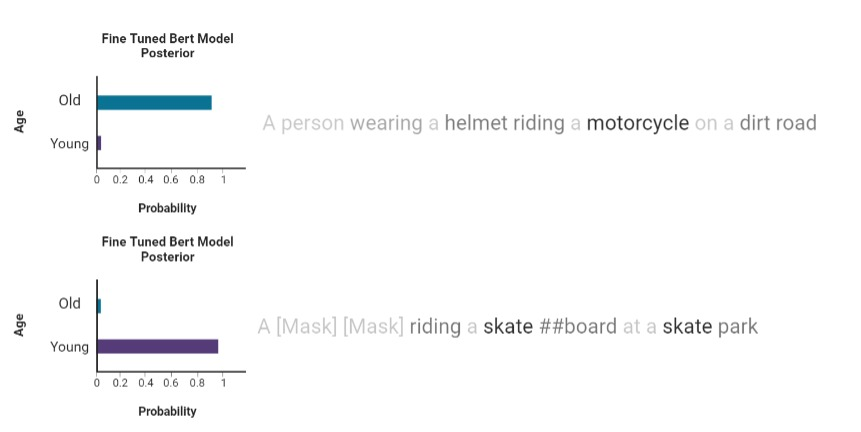
\includegraphics[width= 30em]{images/young-old.jpeg}
    \caption{Captions and confidence levels predicted as ``old'' and ``young'' by the BERT model trained on the age dataset. Darker hue indicates larger attention weight.}
    \label{fig:old}
\end{figure}

\begin{figure}[h]
    \centering
    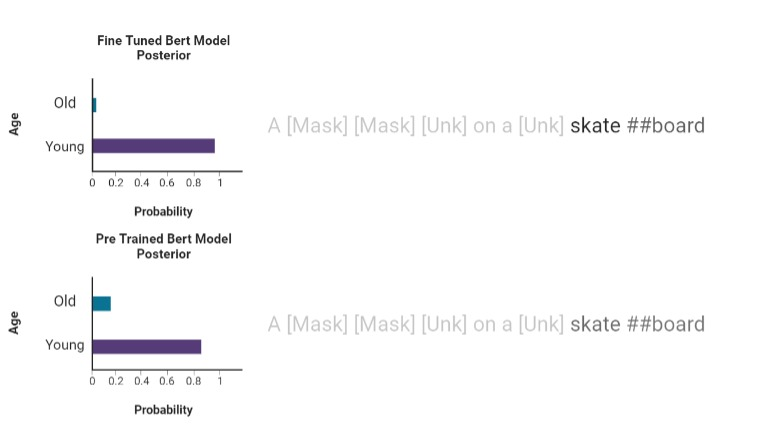
\includegraphics[width=22em]{images/fine-pre.jpeg}
    \caption{Attention maps and confidence levels for BERT-ft and BERT-pre trained on the age dataset. Darker hue indicates larger attention weight.}
    \label{fig:vs}
\end{figure}

\section{Discussion}
\label{sec:discussion}
%Give your judgement on if your experimental results support the claims of the paper. Discuss the strengths and weaknesses of your approach - perhaps you didn't have time to run all the experiments, or perhaps you did additional experiments that further strengthened the claims in the paper.
% we have young words and old words, for each caption we check if it contains a young word or old word. if it contains young OR (young and old) then we say young. If there are old words, we say old. If there are none, we say "unknown"$
\subsection{Main claims}
The reproduced results reproducing are slightly different from the original paper's results. One reason for this is only training the classifiers with 3 seeds per model instead of 10 due to limited computational resources. Our results are therefore slightly less reliable. Even though the numbers are different, our results support all four main claims from the original paper. 

When inspecting the results, it is remarkable that for all protected attributes, BERT-ft generally has the lowest LIC score in comparison to the other classifiers. Specifically, the $LIC_D$ scores for BERT-ft are higher, indicating that this classifier learns to predict the protected attribute better from a masked human caption. While the $LIC_M$ scores for BERT-ft are also higher, showing that BERT-ft is the best performing classifier in general, the increase in $LIC_D$ is larger than for $LIC_M$, resulting in a lower LIC score. BERT-ft's proficiency in learning the dataset bias is attributed to its attention mechanism having been adjusted to the dataset during the finetuning stage.

%\begin{itemize}
%    \item interpret results of original paper's reproduction, comment on numbers in tables and attribute reasons for why they are like that (e.g. why BERT-ft has lowest LIC, why $LIC_D$ is higher in BERT-ft etc). IMPORTANT TO SAY BERT-ft  has higher $LIC_D$ scores, which shows that this encoder learns the bias in the dataset better.
%    \item discuss how our reproduced results are not foolproof: using only 3 seeds, less computational resources, no access to original paper's weights - ie limitations of reproduction (but not all of them just the big ones)

%    \item move on to extension: how our extension backs up original results and claims (age and attention maps)
%    \item how our extension contradicts main claims (age and attention maps)
%    \item how our extension is not fully comparable to original work (AKA limitations): we used a non-specific dataset, we have the [mask][mask] adjective problem etc)
%\end{itemize}
%Then continue with the other points from the blackboard.


\subsection{Encoder analysis using attention visualizer}

Visualizing the attention heads of each encoder layer allows us to observe which tokens of a caption are strongly correlated with the class token. We performed a qualitative analysis on the attention heads of the pretrained and finetuned BERT models using our implemented attention visualizer. Thus we make sure that the two BERT encoders act as expected in two ways: they should not look at the masked words to make predictions, and the correlation between the detected class and the words associated with a class should be strong.
%After inspecting multiple layers' attention heads, we found one attention head in the fourth layer that shows a strong correlation between the class token and bias-related words. In the age experiment, the young class is strongly coupled to words such as ``skateboard", and the old class is strongly associated with words such as ``motorcycle". Figure \ref{fig:old} illustrates this association, and the confidence level is very high for the correct class when such a class-related word is present.
The results of our qualitative analysis show that the models indeed pay attention to the words we expect them to look at. This is illustrated in Figure \ref{fig:old}.

Figure \ref{fig:vs} illustrates how the attention weights of BERT are adapted to the task, showing that the finetuned encoder manages to turn its attention to class-hinting tokens much better than the pretrained one. This analysis allows us to understand why the finetuned BERT performs better than the other encoders. The advantage of finetuned attention is also visible in the confidence scores of the prediction, with the pretrained BERT being less confident (albeit still correct) with its predicted class. 


\subsection{Reviewing LIC and the original claims about it in the age context} %TODO change subsection name
The results obtained for the age experiments can be attributed to a number of key factors. Firstly, there appears to be bias mitigation in multiple models and under the use of multiple encoders, which cannot be said about the reproduced experiments. The high values of the $LIC_D$ scores are mostly responsible for this, seeing as the other component of the LIC score, the model bias, does not appear to have changed from the other experiments. As such, we attribute the bias mitigation effect to the encoders being more capable of learning the bias in the dataset. This effect can also be attributed to the age attribute being mostly expressed as an adjective. Due to this syntactic trait, the bias can be learnt with more ease.

To re-evaluate the authors' claims using the information gathered from the extension experiment, we first look at claims 1 and 2, which state that all models amplify racial and gender bias. As has been discussed, age bias does not appear to be amplified by all models. 
%The multidude of negative LIC scores shows that indeed not all models amplify age bias. 
Instead, only UpDn, Transformer and Oscar appear to amplify age bias.

LIC's robustness against encoders was also further tested in our extension. This can be evaluated by observing whether it fluctuates for one model depending on the employed encoder. In the age experiment's case, we notice some minor fluctuations in some models, but generally the LIC scores for the three encoders have the same polarity. Keeping in mind we already discussed how  BERT-ft learns the bias in the dataset better, so slightly different results are to be expected, we maintain the claim that LIC is robust against encoders. 

\subsection{Limitations of age experiment}
While the age attribute has significantly contributed to our understanding and confidence in the claims from the main paper, it must be noted that this experiment also has some weaknesses. Besides the smaller dataset size, the used captions dataset was not even specialized for the age experiment. Instead, the gender dataset was used. A dataset built specifically for age bias experiments would be more suitable for the task, and should result in more valuable findings. Moreover, the attribute masking was done automatically for this experiment, and it did not perform without issues. When consecutive words contained information about the protected attribute, multiple masks were applied. Therefore, some sentences contained two concatenated mask tokens, instead of simply using one mask token. Due to the stochasticity of the models used in the experiments, it is highly probable that using one mask token for multiple words would lead to different results. 

\subsection{What was easy} % farrukh
%Give your judgement of what was easy to reproduce. Perhaps the author's code is clearly written and easy to run, so it was easy to verify the majority of original claims. Or, the explanation in the paper was really easy to follow and put into code. 
%Be careful not to give sweeping generalizations. Something that is easy for you might be difficult to others. Put what was easy in context and explain why it was easy (e.g. code had extensive API documentation and a lot of examples that matched experiments in papers).

\subsubsection{Operational code} The base code ran right out of the box, and required no modification on our part to make it operational.
\vspace*{-0.5cm}
\subsubsection{Hyperparameters} The hyperparameters used to train models were clearly provided in the supplementary materials section for all model configurations.
\vspace*{-0.5cm}
\subsubsection{Data availability} The data is linked by the author, and the instructions for where to place it were clear and allowed for a quick setup.
\vspace*{-0.5cm}
\subsubsection{Run arguments} The provided scripts have an extensive argument parser, making it easy to modify relevant fields such as the captions dataset, hyperparameter settings, and random seeds. This allowed us to quickly set up our experiments.

%The authors provided \textbf{fully functional code} that required no modification to work. \textbf{Hyperparameters} were also provided for each model's configurations. The \textbf{datasets were available} and clear instructions on how to use them with the code were offered. Lastly, the code's \textbf{argument parser} made it easy to understand the purpose of each argument and how to change them to match every experiment's requirements.

\subsection{What was difficult} \label{sec:difficult}% farrukh

% 1. uncommented code (descriptive variable names at least)
% 2. code is difficult to extend
\subsubsection{Lack of comments} % The provided code exhibits numerous poor coding practices. Most noticably, the code contains little to no comments, which causes difficulties when interpreting it. 
The provided code's documentation contains room for improvement. As a result, we had difficulties interpreting it.
\vspace*{-0.5cm}
\subsubsection{Repetitive code}
The scripts for the gender and race attributes and different encoders are very similar. Extending the code mainly involved duplicating the BERT and LSTM gender scripts and modifying them by changing relevant keywords/variable names, which is not an optimal way of adding new attributes. 
%These can be greatly simplified by utilizing imports and writing object classes. 
% 3. too many seeds to train
%\subsubsection{Limited computational resources} The original paper's experiments were conducted with 10 seeds. We could only conduct experiments with 3 due to a lack of computational sources, meaning our results are less precise compared to the ones we were trying to reproduce.

% 4. impossible to interpret classifier model and understand why LIC is the way it is
%\subsubsection{Uninterpretable classifier} The original paper utilizes no methods of explaining how the classifier determines which features to 

\vspace*{-0.5cm}
% 5. Model weights unavailable
\subsubsection{Unavailable model weights} The authors retrained all image captioning models on only the MSCOCO training dataset, as they intended to use the validation set for evaluation. However, the retrained model weights were not available. As a result, we had to use the generated captions provided by the authors instead of generating them ourselves.


%List part of the reproduction study that took more time than you anticipated or you felt were difficult. 

%Be careful to put your discussion in context. For example, don't say "the maths was difficult to follow", say "the math requires advanced knowledge of calculus to follow". 

\subsection{Communication with original authors}
%Document the extent of (or lack of) communication with the original authors. To make sure the reproducibility report is a fair assessment of the original research we recommend getting in touch with the original authors. You can ask authors specific questions, or if you don't have any questions you can send them the full report to get their feedback before it gets published. 
We did not communicate with the original authors, neither about our reproduction of their paper nor about the extensions that we implement and test.

% \subsection{Conclusion} %dk if we need one